%In an EDGE block, data dependent instructions do not pass data to each other via reads and writes to registers, instead the result of an instruction is passed to the operands of instructions who depend on the data (see Chapter~\ref{chp:Background} Section~\ref{sec:edge_isa} for more information).
In the EDGE architecture registers are primarily used to pass values between blocks, which can cause data dependencies.
In a core composition the register files of each core in the composition becomes distributed (Chapter~\ref{chp:Background} Section~\ref{chp:Background:sec:EDGE}) to ensure that each core has the same view of the current execution state.
An example of values passed between blocks is the loop induction variable of the loop in Listing~\ref{lst:basic2}.% are going to be passed via 3 registers in the block that represents the body of the loop.
If this loop is executing on a 16 core composition, then one of the cores will have to issue all the reads to this register for all other cores.
This of course will put stress on the NoC, and increase the latency of what is meant to be a fast instruction.

%The register files becomes distributed and each core becomes responsible for a set of registers; for example in a 2 core composition, the even numbered registers are handled by Core 0 whilst the even number registers are handled by Core 1.
%This means that when Core 1 wants to read or write to Register 0 it must send a request via the network on chip (NoC) as this register is located on Core 0.

\begin{figure}[t]
\lstset{language=C,numbersep=4pt}
\centering
\begin{lstlisting}
	for(int i =0 ; i < 100000; i++)
		a[i] = c[i]*b[i];
\end{lstlisting}
\captionof{lstlisting}{Example of small loop.}\label{lst:basic2}
\vspace{2em}
    \centering
    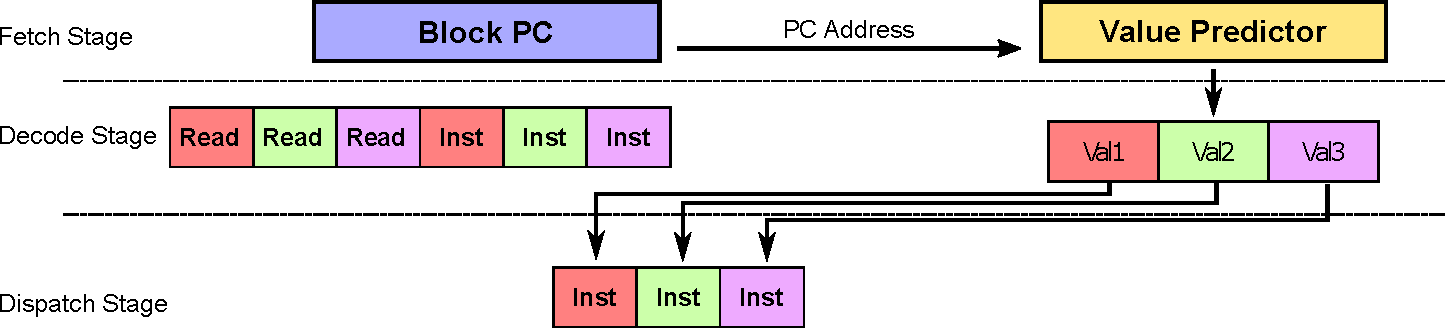
\includegraphics[width=1\textwidth]{chapter3/graphics/val_pred_overview.pdf}
    \captionof{figure}{Overview of how a value predictor should work for EDGE. Prediction is made at the fetch stage, and predictions are used when register reads are dispatched.}
    \label{fig:bad_overview}
\vspace{1em}
\end{figure}

To ensure that a younger block does not execute a read to a register that must be written to by an older block, the register-file keeps track of registers which will be written to by older blocks.
If the younger block attempts to execute the read, its request is pushed back until the older block has executed its write and any instruction that depends on the read must wait until the write fires.
Whilst the serialisation of register reads and writes between blocks ensures correct execution of speculative blocks, it effectively reduces the potential for instruction level parallelism (ILP).
This is further exacerbated when fusing a large number of cores, as this increases the number of blocks that may have to wait on register reads and writes.

This chapter underlines two problems related to register reads on large compositions: the potential data dependencies caused by reads waiting for previous writes to execute, and the latency caused by having to send read requests via the NoC.
The problem of trying to reduce register and memory dependencies to improve instruction level parallelism is not new, and is an issue found in more traditional out of order superscalar processors~\cite{peraisVTAGE2014}.

For example, in the loop of Listing~\ref{lst:basic}, the sole data dependency is found in the loop induction variable.
This variable is always incremented by 1, which means that given a block, the value can easily be predicted based on previous values of the variable.
The other register values, such as the memory bases can also be predicted as they never change.
If each core is able to predict the value of the register reads, then they can speculatively execute instructions that depend on these registers before the real value arrives.
In these cases value prediction can be used to attempt to ensure that these blocks can run in parallel even if there are dependencies.


\subsection{Design features of a value predictor}

In this chapter, the only target for value prediction is register read instructions.
This is due to the fact that they are prime suspects for data dependencies and unlike loads, currently cannot be fired speculatively.
Ideally, a value predictor for EDGE would function as seen in Figure~\ref{fig:bad_overview}.
When a block is fetched, a single request is made to the value predictor to fetch all predictions for the read instructions of the block.
At dispatch time, the predicted values are used and forwarded to dependent instructions, whilst the read instructions are issued.
This allows the depending instructions to execute whilst the reads are still being processed.
%This section covers different features that must be considered when implementing such a value predictor.


\paragraph*{Prediction Latency}
In a traditional superscalar processor, one of the main challenges value predictors face is being able to sustain the potential number of prediction requests in a short time frame~\cite{peraisBeBop2015}.
As value predictors are designed to improve ILP performance it is important to be able to issue a predicted value quickly.
If multiple prediction requests are made each cycle, this requires expensive hardware such as a re-order buffer to hold all predictions~\cite{peraisBeBop2015}.

To tackle the challenge of issuing predictions quickly, research has focused on grouping predictions into blocks~\cite{peraisBeBop2015}.
Instead of issuing a request per instruction a single prediction, the predictor receives a single request for a set of instructions in a basic block.
Entries are accessed by using the PC of the first instruction of the fetch block.
By grouping multiple predictions into a single entry, it drastically reduces the number of requests to the value predictor, reducing the prediction latency for a large number of instructions.
As EDGE organises instructions as blocks, a block-based predictor would reduce the number of prediction requests per cycle, making it an attractive feature.

%Rewrite
\paragraph*{Prediction generation} Another important feature when selecting a value predictor is how it generates a predicted value.
Currently, there exist two methods: \textit{context} value prediction~\cite{peraisVTAGE2014} and \textit{computational} value prediction~\cite{peraisBeBop2015,gabbayVPOrig,goeman01dfcm}.
More details on how these two predictors differ can be found in Chapter~\ref{chp:Background} Section~\ref{sec:valpred}.
To summarise, \textit{context} predictors simply fetch a value from a table to generate a prediction, whilst \textit{computational} calculate the predicted variable.

Whilst \textit{context} predictors are simpler to design, as there are no extra functions required to generate the predictions aside from fetching a value from a table, they are often considered less efficient when used in loops~\cite{peraisBeBop2015}.
For example, the memory address of an item in an array from Listing~\ref{lst:basic2} is always incremented using a fixed stride (the loop induction increment).
In order for a \textit{context} value predictor to correctly predict the address, it must already be stored in its table.
Multiple values for a single instruction must be stored in the table in order to predict the different addresses throughout the execution of the loop.
Having a large number of values stored in the predictor for a single instruction is inefficient, unless the predictor is very large.

On the other hand, a \textit{computational} predictor can capture how the memory address changes each iteration by determining the \textit{stride} at which it is modified.
This means that a \textit{computational} predictor will only have to store 2 values: one for the stride and another for the last committed value.
Not only does this reduce the number of entries a single instruction occupies in the predictor, but it allows a \textit{computational} predictor to generate predictions faster than the \textit{context} predictor since the next memory address will be equal to $ lastCommittedValue + stride$.

Core composition is often most effective when executing over loops, as seen throughout chapter~\ref{chp:cases}.
As variables such as loop inductors are passed between blocks via register reads and writes, they are a prime candidate for value prediction.
Since these variables are often modified using the same stride throughout the loop and the loops may occur multiple times during the execution of the program it is important that the predictor keeps the least amount of information for each value.
This is to ensure that multiple values can co-exist in the predictor, increasing the overall coverage.
\textit{Computational} predictors are therefore more adequate for this scenario, as they require fewer entries to predict a single value and are able to generate predictions faster.


\paragraph*{Summary}

A value predictor for EDGE must be able to provide predictions in groups, as EDGE organises its instructions in blocks as this reduces the number of prediction requests per block.
As core composition is mostly used to improve the performance of loops, a \textit{computational} predictor is more adequate than a context based one.
Perais {\it et al.~}propose such a predictor: a block based differential Value TAGE predictor~\cite{peraisBeBop2015}.
The next section covers briefly how this predictor works, however more details can be found in Chapter~\ref{chp:Background} Section ~\ref{sec:valpred}.

\subsection{Block-based D-VTAGE predictor}

In this chapter, a \textit{block} based differential value TAGE (D-VTAGE) predictor is implemented, based on the work of Perais {\it et al.~}~\cite{peraisBeBop2015}.
Full details on how such a value predictor works can be found in Chapter~\ref{chp:Background} Section~\ref{chp:bck:vtage}.
To summarise, D-VTAGE is a \textit{computational} based value predictor: a prediction is composed of the last seen value for the instruction (found in a Last Value Table (LVT)), and a stride which represents the delta between the last two values for the instruction.
When a prediction is made, the last seen value and stride are added together to make the predicted value.
Unlike a traditional value predictor that issues 1 prediction per instruction, this predictor issues multiple predictions at a time (\textit{blocks} of predictions).
Predictions are validated during the commit phase of a block~\cite{peraisVTAGE2014}.
This is achieved by comparing the predicted values with the real values read from the registers.
In case of a misprediction, a pipeline squash is issued for all blocks younger than the mispredicting block.
The mispredicting block is then re-executed, this time without value prediction.

The predictor also handles the fact that multiple blocks may be in flight, and thus the value found in the LVT may not be up to date.
This is done via a speculative window that has its own LVT that is speculatively updated when new predictions are made.
This allows the predictor to be able to handle situations where multiple iterations of a loop are in flight.
Since EDGE blocks are single entry, there is no need for a complicated update mechanism for the Speculative Window as defined in~\cite{peraisBeBop2015}.
When a block is flushed, it is also removed from the speculative window.

%Instead of issuing a single prediction per request, the block based D-VTAGE predictor issues multiple predictions for a single request.
%This is an ideal mechanism when considering EDGE is the targeted platform.
%In this case, when an EDGE block is fetched, a single request has to be made to the predictor to fetch all predictions for register reads.

%Finally, as EDGE blocks are single entry, multiple exits, this simplifies the update mechanism for the Speculative Window.
%In the original proposal of D-VTAGE by Perais {\it et al.~}~\cite{peraisBeBop2015} they discuss the issue of how to handle updates in the Speculative Window after a flush.
%This is due to the fact that in a traditional x86 environment, instructions being fetched after a flush may belong to a block of instructions that initiated the flush.
%As this is not possible in EDGE, since whole blocks are flushed and fetched, there is no need for a complicated update policy.
%Instead, a new prediction is always made when a block is fetched.



%\subsection{Perfect Value Predictor}

%The perfect value predictor is implemented using traces of the application being executed.
%When a new block is fetched, it querries the trace file and looks for the values of all the registers which will be read.
%When the block can execute a read, the simulator then feeds the register directly into the instruction operands, instead of querying the register file.

%The perfect value predictor has no hardware restriction as to fully capture the potential performance improvements.
%Thus, all the registers in a block can be predicted.
%More on how restricting the number of values which can be predicted per block is discussed in the analysis in Section~\ref{chp:chp3:sec:analysis}.
